% !TEX enableShellEscape = yes
% (The above line makes atom's latex package compile with -shell-escape
% for minted, and is just ignored by other systems.)
\documentclass{article}

\usepackage{fullpage}
\usepackage{color}
\usepackage{amsmath,amssymb}
\usepackage{url}
\usepackage{verbatim}
\usepackage{graphicx}
\usepackage{parskip}
\usepackage{amssymb}
\usepackage{hyperref}

% Use one or the other of these for displaying code.
% NOTE: If you get
%  ! Package minted Error: You must invoke LaTeX with the -shell-escape flag.
% and don't want to use minted, just comment out the next line
\usepackage{minted} \BeforeBeginEnvironment{minted}{\begingroup\color{black}} \AfterEndEnvironment{minted}{\endgroup} \setminted{autogobble,breaklines,breakanywhere,linenos}

\usepackage{listings}

% Colours
\definecolor{blu}{rgb}{0,0,1}
\newcommand{\blu}[1]{{\textcolor{blu}{#1}}}
\definecolor{gre}{rgb}{0,.5,0}
\newcommand{\gre}[1]{\textcolor{gre}{#1}}
\definecolor{red}{rgb}{1,0,0}
\newcommand{\red}[1]{\textcolor{red}{#1}}
\definecolor{pointscolour}{rgb}{0.6,0.3,0}

% answer commands
\newcommand\ans[1]{\par\gre{Answer: #1}}
\newenvironment{answer}{\par\begingroup\color{gre}Answer: }{\endgroup}
\let\ask\blu
\let\update\red
\newenvironment{asking}{\begingroup\color{blu}}{\endgroup}
\newcommand\pts[1]{\textcolor{pointscolour}{[#1~points]}}

% Math
\def\R{\mathbb{R}}
\DeclareMathOperator*{\argmax}{arg\,max}
\DeclareMathOperator*{\argmin}{arg\,min}
\newcommand{\norm}[1]{\lVert #1 \rVert}
\newcommand{\mat}[1]{\begin{bmatrix}#1\end{bmatrix}}

% LaTeX
\newcommand{\fig}[2]{\includegraphics[width=#1\textwidth]{#2}}
\newcommand{\centerfig}[2]{\begin{center}\includegraphics[width=#1\textwidth]{#2}\end{center}}

\begin{document}


\title{CPSC 340 Assignment 6}
\date{}
\maketitle

\vspace{-7em}



\section*{Important: Submission Format \pts{5}}

Please make sure to follow the submission instructions posted on the course website.
\ask{We will deduct marks if the submission format is incorrect, or if you're not using \LaTeX{} and your submission is \emph{at all} difficult to read} -- at least these 5 points, more for egregious issues.
Compared to assignment 1, your name and student number are no longer necessary (though it's not a bad idea to include them just in case, especially if you're doing the assignment with a partner).

\vspace{1em}

\section{Robust PCA for Background Subtraction}

If you run \verb|python main -q 1|, the program will load a dataset $X$ where each row contains the pixels from a single frame of a video of a highway. The demo applies PCA to this dataset and then uses this to reconstruct the original image.
It then shows the following 3 images for each frame:
\begin{enumerate}
	\item The original frame.
	\item The reconstruction based on PCA.
	\item A binary image showing locations where the reconstruction error is non-trivial.
\end{enumerate}
Recently, latent-factor models have been proposed as a strategy for ``background subtraction'': trying to separate objects from their background. In this case, the background is the highway and the objects are the cars on the highway.

Why does this make any sense? Remember that PCA tries to find principal components that reconstruct the dataset well. Here the training examples are highway images. Now, we need to reconstruct these highway images out of a small number of PC images. Since we want to reconstruct them well, we're going to create PCs that capture the \emph{common features across the entire dataset}. In other words, the PCs will try to reconstruct the highway and slight variations of the highway, because that is always there. If a car appears in the top-left of only a couple images, we might not want a PC for that case, since that PC is useless for the majority of the training set. Thus, when we try to reconstruct the images we are left to see only the parts of the image that can be made out of the PCs, or in other words that are common across all the images. Hence why the reconstructions look like the background. We can then subtract this reconstruction (background) from the original image to get objects of interest (foreground). Cool, right?

In this demo, we see that PCA does an OK job of identifying the cars on the highway in that it does tend to identify the locations of cars. However, the results aren't great as it identifies quite a few irrelevant parts of the image as objects. Who likes good news --- everyone? Well good news, everyone! We can use robust PCA to do even better.

Robust PCA is a variation on PCA where we replace the L2-norm with the L1-norm,
\[
f(Z,W) = \sum_{i=1}^n\sum_{j=1}^d |\langle w^j, z_i\rangle - x_{ij}|,
\]
and it has recently been proposed as a more effective model for background subtraction.

\subsection{Why Robust PCA \pts{5}}

\ask{In a few sentences, explain why using a robust loss might help PCA perform better for this background subtraction application.} Some conversation-starters: what is an outlier here --- a car or the highway? What does it mean to be robust to outliers --- that we're good at reconstructing them or that we're back at reconstructing them?
\begin{answer}
	In the case of car and highway, the outlier is the car. If we punish severely on the exsistence of outliers, then the code will force the car and the highway mixing together, resulting in something blurry and bad for background subtraction.
	
	If we, instead, use the robust loss, we are more tolerent to outliers, and less accurate on reconstructing. In this way, the code can to some extent ignore the car and focus on reconstructing the highway only.
\end{answer}
\subsection{Robust PCA Approximation and Gradient \pts{5}}

If you run \verb| python main.py -q 1.3 |, the program will repeat the same procedure as in the above section, but will attempt to use the robust PCA method, whose objective functions are yet to be implemented. You will need to implement it (yay!).

We'll use a gradient-based approach to PCA and a smooth approximation to the L1-norm. In this case the log-sum-exp approximation to the absolute value may be hard to get working due to numerical issues. Perhaps the Huber loss would work. We'll use the ``multi-quadric'' approximation:
\[
|\alpha| \approx \sqrt{\alpha^2 + \epsilon},
\]
where $\epsilon$ controls the accuracy of the approximation (a typical value of $\epsilon$ is $0.0001$). Note that when $\epsilon=0$ we revert back to the absolute value, but when $\epsilon>0$ the function becomes smooth.

Our smoothed loss is:

\[
f(Z,W) = \sum_{i=1}^n\sum_{j=1}^d \sqrt{(\langle w^j, z_i\rangle - x_{ij})^2 + \epsilon }
\]

The partial derivatives of this loss with respect to the elements of $W$ are
(\update{this derivation has been corrected since first posting, though the final answer was always right}):

\begin{align*}
\frac{\partial}{\partial w_{cj}} f(Z,W)
  &= \frac{\partial}{\partial w_{cj}} \sum_{i=1}^n\sum_{j'=1}^d \left( (\langle w^{j'}, z_i\rangle - x_{ij'})^2 + \epsilon \right)^{\frac12} \\
  &= \sum_{i=1}^n \frac{\partial}{\partial w_{cj}} \left( (\langle w^{j}, z_i\rangle - x_{ij})^2 + \epsilon \right)^{\frac12}  \qquad \text{(since the $j' \ne j$ terms have no $w_{cj}$ in them)} \\
  &= \sum_{i=1}^n \frac12 \left( (\langle w^{j}, z_i\rangle - x_{ij})^2 + \epsilon \right)^{-\frac12} \frac{\partial}{\partial w_{cj}} \left( (\langle w^{j}, z_i\rangle - x_{ij})^2 + \epsilon \right) \\
  &= \sum_{i=1}^n \frac12  \left( (\langle w^{j}, z_i\rangle - x_{ij})^2 + \epsilon \right)^{-\frac12} \;2\,  (\langle w^{j}, z_i\rangle - x_{ij}) \; \frac{\partial}{\partial w_{cj}} \langle w^{j}, z_i\rangle \\
  &= \sum_{i=1}^n \left( (\langle w^{j}, z_i\rangle - x_{ij})^2 + \epsilon \right)^{-\frac12}  (\langle w^j, z_i\rangle - x_{ij}) \, z_{ic}
\end{align*}

The partial derivatives with respect to $Z$ are similar:

\begin{align*}
\frac{\partial}{\partial z_{ic}} f(Z,W)
  &= \frac{\partial}{\partial z_{ic}} \sum_{i'=1}^n \sum_{j=1}^d  \left( (\langle w^j, z_{i'}\rangle - x_{i'j})^2 + \epsilon \right)^{\frac12}\\
  &= \sum_{j=1}^d  \left( (\langle w^j, z_{i}\rangle - x_{ij})^2 + \epsilon \right)^{-\frac12}   (\langle w^j, z_{i}\rangle - x_{ij}) \; \frac{\partial}{\partial z_{ic}} \langle w^j, z_i\rangle \\
  &= \sum_{j=1}^d  \left( (\langle w^j, z_i\rangle - x_{ij})^2 + \epsilon \right)^{-\frac12}  (\langle w^j, z_i\rangle - x_{ij}) \, w_{cj}
\end{align*}

If we put this into matrix(ish) notation, we get the following:

\[
\nabla_W f(Z,W) = Z^T \left[ R \oslash \left(R^{\circ 2} + \epsilon\right)^{\circ \frac12}  \right]
\]

where $R\equiv ZW-X$,
$A \oslash B$ denotes \textbf{element-wise} division of $A$ and $B$,
$A + s$ for a scalar $s$ denotes element-wise adding $s$ to each entry of $A$,
and $A^{\circ p}$ denotes taking $A$ to the \textbf{element-wise} power of $p$.

And, similarly, the gradient with respect to $Z$ is given by:

\[
\nabla_Z f(Z,W) = \left[ R \oslash \left(R^{\circ 2} + \epsilon\right)^{\circ \frac12} \right] W^T
\]

\ask{Show that the two parts of the gradient above, $\nabla_W f(Z,W)$ and $\nabla_Z f(Z,W)$, have the expected dimensions.}
\begin{answer}
	First, let's look at $\nabla_W f(Z,W)$. Since all computations in $\left[ R \oslash \left(R^{\circ 2} + \epsilon\right)^{\circ \frac12}  \right]$ is element-wise, the result of this part should be in the same dimension as $R$ and essentially the same as $X$, i.e. $n \times d$. We also know $Z^T$ is $k \times n$, so the final result should be a $k \times d$ matrix, which is the expected dimension since W is $k \times d$.

	Similarly, for $\nabla_Z f(Z,W)$, $\left[ R \oslash \left(R^{\circ 2} + \epsilon\right)^{\circ \frac12} \right]$ will generate a $n \times d$ matrix. $W^T$ is $d \times k$. Therefore, the final result is $n \times k$, the same dimension as $Z$ as expected.
\end{answer}

\subsection{Robust PCA Implementation \pts{10}}

In \texttt{fun\_obj.py}, you will find classes named \texttt{RobustPCAFactorsLoss} and \texttt{RobustPCAFeaturesLoss} which should compute the gradients with respect to $W$ and $Z$, respectively. \ask{Complete the \texttt{evaluate()} method for each using the smooth approximation and gradient given above. Submit (1) your code in \texttt{fun\_obj.py}, and (2) one of the resulting figures.}

Hint: Your code will look similar to the already implemented \texttt{PCAFactorsLoss} and \texttt{PCAFeaturesLoss} classes. Note that the arguments for \texttt{evaluate()} are carefully ordered and shaped to be compatible with our optimizers.

Note: The robust PCA is somewhat sensitive to initialization, so multiple runs might be required to get a reasonable result.
\begin{answer}
	

	\begin{minted}[]{python}
	class RobustPCAFeaturesLoss(FunObj):
		def __init__(self, epsilon):
			self.epsilon = epsilon

		def evaluate(self, z, W, X):
			n, d = X.shape
			k, _ = W.shape
			Z = z.reshape(n, k)

			R = Z @ W - X
			R_2 = np.sqrt(R ** 2 + self.epsilon)
			RR = R / R_2
			f = np.sum(R_2) 
			g = RR @ W.T
			return f, g.flatten()

	class RobustPCAFactorsLoss(FunObj):
		def __init__(self, epsilon):
			self.epsilon = epsilon

		def evaluate(self, w, Z, X):
			n, d = X.shape
			_, k = Z.shape
			W = w.reshape(k, d)

			R = Z @ W - X
			R_2 = np.sqrt(R ** 2 + self.epsilon)
			RR = R / R_2
			f = np.sum(R_2)
			g = Z.T @ RR
			return f, g.flatten()
	\end{minted}

	\begin{figure}[htbp!]
		\centering
		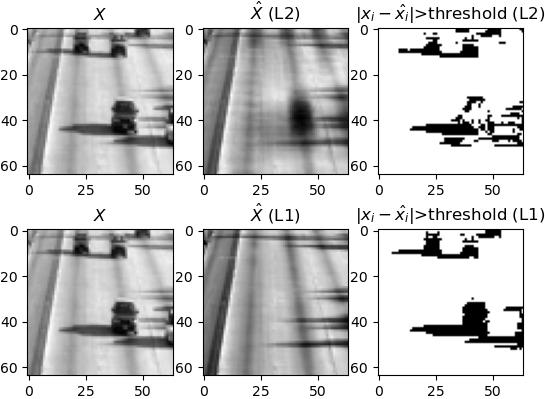
\includegraphics[width = .7\textwidth]{figs/robustpca_highway_003.jpg}
	\end{figure}
\end{answer}


\subsection{Reflection \pts{6}}

\begin{enumerate}
	\item Very briefly comment on the results from the previous section --- does robust PCA seem to do better than regular PCA for this task?
	\begin{answer}
		From the figure, the robust result seems to better differentiate the cars and the highway.
	\end{answer}
	\item How does the number of video frames and the size of each frame relate to $n$, $d$, and/or $k$?
	\begin{answer}
		$n$ represents the number of video frames, $d$ refers to the size of rach frame. $k$ is selected by programmer, which is not related to the frames as long as $k < d$ 
	\end{answer}
	\item What would the effect be of changing the threshold (see code) in terms of false positives (cars we identify that aren't really there) and false negatives (real cars that we fail to identify)?
	\begin{answer}
		A higher threshold will give more false negatives but fewer false positives.
	\end{answer}
\end{enumerate}


\clearpage
\section{Movie Recommendations}

If you run \texttt{python main.py -q 2}, the program will perform the following steps:

\begin{enumerate}
\item Loads the small educational version of the MovieLens dataset (\url{https://grouplens.org/datasets/movielens/}).
\begin{answer}
	
\end{answer}

\item Prints out the first 5 rows of the ratings dataframe (which we'll use) and the movies dataframe (which we won't use, but is loaded FYI).

\item Transforms the ratings table into the $Y$ matrix described in lecture.

\item Splits $Y$ into train (80\% of the ratings) and validation (20\% of the ratings) matrices.

\item Prints out some stats about the dataset, including the average rating in the training set.

\end{enumerate}

\subsection{Understanding $Y$ \pts{6}}

\ask{Answer the following questions:}

\begin{enumerate}
\item In lecture, we used the ``?'' symbol to represent missing ratings. How are these missing entries of $Y$ implemented in the code?
\item How many (non-missing) ratings are there in \texttt{Y\_train} and \texttt{Y\_valid}, respectively?
\item Does the same user-movie rating ever appear in \emph{both} \texttt{Y\_train} and \texttt{Y\_valid}? Is the result as expected?
\end{enumerate}


\subsection{Implementing Collaborative Filtering \pts{15}}

If you run \texttt{python main.py -q 2.2}, the code will fit a model that doesn't actually do anything. It uses the same alternating minimization scheme as in the previous question on Robust PCA. \ask{Fill in the \texttt{evaluate} methods of the \texttt{CollaborativeFilteringWLoss} and \texttt{CollaborativeFilteringZLoss} classes in \texttt{fun\_obj.py}. Submit your code.}

Hint: Since we're minimizing the regularized PCA loss, your code should be quite similar to the \texttt{evaluate} methods in \texttt{PCAFeaturesLoss} and \texttt{PCAFactorsLoss}. I suggest you copy/paste those methods as a starting point. However, there are two changes you'll need to make: (1) modify the loss and gradient to account for the regularization, and (2) accounting for the fact that the loss should only sum over the available ratings, not the entire $Y$ matrix. The easiest way to account for this is to modify the $R$ matrix by setting all its NaN values to 0. Since $R$ represents the residuals (or reconstruction errors), setting these to 0 says that these entries don't contribute to the loss, which is exactly what we want.



\subsection{Hyperparameter tuning \pts{5}}
If you run \texttt{python main.py -q 2.3}, the program will implement a baseline model that predicts the average rating (around 3.5 stars) for all missing ratings.
As you'll see from the output, this baseline has a root mean squared error (RMSE) of slightly above 1 star. The hyperparameters we gave you in the code actually do worse than this (my validation RMSE is around 1.3 stars). \ask{Adjust the hyperparameters of your collaborative filtering model, namely $k,\lambda_W,\lambda_Z$, until you obtain a better validation error than the baseline. Submit the hyperparameters you found as well as your training and validation RMSE.}

PS: there is nothing to stop you from just guessing random hyperparameters, but it would be cool if you think about the fact that the current model overfits and adjust each of the hyperparameters in the direction that reduces the complexity of the model to combat the overfitting.


\subsection{Regularization with PCA \pts{5}}

In lecture we discussed the fact that with regularized PCA, we need to regularize both $W$ and $Z$ for things to make sense. Test this out empirically by setting $\lambda_Z=0$ and $\lambda_W>0$. Modify the code so that it prints out the Frobenius norm of $W$ and $Z$ after each iteration of the alternating minimization (you don't have to submit this printing code though). \ask{Describe your observations and briefly discuss.}


%\clearpage
\section{Neural Networks}

\subsection{Neural Networks by Hand \pts{7}}

Suppose that we train a neural network with sigmoid activations and one hidden layer and obtain the following parameters (assume that we don't use any bias variables):
\[
W = \mat{-2 & 2 & -1\\1 & -2 & 0}, v = \mat{3 \\1}.
\]
Assuming that we are doing regression, \ask{for a training example with features $x_i^T = \mat{-4 &-2 & 4}$ what are the values in this network of $z_i$, $h(z_i)$, and $\hat{y}_i$?}

\subsection{Neural Networks vs. Linear Classifier \pts{7}}

%\textbf{NOTE}: before starting this question you need to download the MNIST dataset from \\ \url{http://deeplearning.net/data/mnist/mnist.pkl.gz} and place it in your \emph{data} directory.

If you run \texttt{python main.py -q 3}, the program will train a multi-class logistic regression classifier on the MNIST handwritten digits data set using stochastic gradient descent with some pre-tuned hyperparameters.
The scikit-learn implementation called by the code uses a minibatch size of 1 and a one-vs-rest strategy for multi-class logistic regression. It is set to train for 10 epochs.
The performance of this model is already quite good, with around 8\% training and validation errors. Your task is to use a neural networks classifier to outperform this baseline model.

If you run \texttt{python main.py -q 3.2}, the program will train a single-layer neural network (one-layer nonlinear encoder paired with a linear classifier) on the same dataset using some pre-tuned hyperparameters. Modify the code, play around with the hyperparameter values (configurations of encoder layers, batch size and learning rate of SGD, standardization, etc.) until you achieve validation error that is reliably below \red{5}\%. \ask{Report (1) the training and validation errors that you obtain with your hyperparameters, and (2) the hyperparameters that you used.}




\subsection{Neural Disentangling \pts{10}}

An intuitive way to think about a neural network is to think of it as a composition of an encoder (all the layers except the last one, including the final nonlinearity) and a linear predictor (the last layer). The predictor signals the encoder to learn a better feature space, in such a way that the final linear predictions are meaningful.

The following figures resulted from running \texttt{python main.py -q 3.3}. For this, a neural network model is used to encode the examples into a 2-dimensional feature space. Here's the original training data:

\centerfig{.7}{./figs/sinusoids.png}

And here is the learned decision boundary of the neural network:

\centerfig{.7}{./figs/sinusoids_decision_boundary_[2]_2.png}

We can look inside and see what the encoder learned. Here is the training data shown in the 2D transformed feature space learned by the encoder (first layer):

\centerfig{.7}{./figs/sinusoids_learned_features_[2]_2.png}

Here is the linear classifier learned by the predictor in this transformed feature space:

\centerfig{.7}{./figs/sinusoids_linear_boundary_[2]_2.png}


This particular neural network solution does not classify the given examples very well. However, if we use a 4-dimensional hidden features (with all else equal), we get a better-looking result:

\centerfig{.7}{./figs/sinusoids_decision_boundary_[4]_2.png}
\centerfig{.7}{./figs/sinusoids_linear_boundary_[4]_2.png}

Note: in this case, since the hidden feature space has dimension 4, we are only able to plot 2 of the 4 dimensions. The actual linear classifiers is a 3D hyperplane dividing the 4D space. However, even with these two dimensions that we can plot, we can already see that the training data looks pretty much linearly separable, and we learn a good classifier.

Previously we changed the \emph{hidden layer size} from 2 to 4. Another change we can make is to increase the \emph{number of layers} from 1 to 2. Let's use 2 layers of hidden features of size 2:

\centerfig{.7}{./figs/sinusoids_decision_boundary_[2, 2]_2.png}
\centerfig{.7}{./figs/sinusoids_linear_boundary_[2, 2]_2.png}

\ask{Answer the following questions and provide a brief explanation for each:}

\begin{enumerate}
	\item Why are the axes ($z_1$ and $z_2$) of the learned feature space scatterplot constrained to $[0, 1]$? Note/hint: here, our definition of $z$ is after the nonlinearity is applied, whereas in the lecture $z$ is defined as before the nonlinearity is applied. Sorry about that!
	%
	\item Does it make sense to use neural networks on datasets whose examples are linearly separable in the original feature space?
	%
	\item Why would increasing the dimensionality of the hidden features (which is a hyper-parameter) help improve the performance of our classifier?
	%
	\item Why would increasing the number of layers help improve the performance of our classifier?
	%
	\item Neural networks are known to suffer problems due to a highly non-convex objective function. What is one way we can address this problem and increase the chances of discovering a global optimum? (Hint: look at the code.)
	%
\end{enumerate}


\section{Very-Short Answer Questions \pts{14}}

\ask{Answer each of the following questions in a sentence or two.}
\begin{enumerate}

\item Give one reason why you might want sparse solutions with a latent-factor model.


\item Which is better for recommending movies to a new user, collaborative filtering or content-based filtering? Briefly justify your answer.


\item{Are neural networks mainly used for supervised or unsupervised learning? Are they parametric or nonparametric?}

\item{Why might regularization become more important as we add layers to a neural network?}


\item{Consider using a fully-connected neural network for 5-class classification on a problem with $d=10$. If the network has one hidden layer of size $k=100$, how many parameters (including biases), does the network have?}


\item What is the ``vanishing gradient'' problem with neural networks based on sigmoid non-linearities?

\item{Convolutional networks seem like a pain... why not just use regular (``fully connected'') neural networks for image classification?}

\end{enumerate}
\end{document}
